% Options for packages loaded elsewhere
\PassOptionsToPackage{unicode}{hyperref}
\PassOptionsToPackage{hyphens}{url}
%
\documentclass[
]{article}
\usepackage{amsmath,amssymb}
\usepackage{iftex}
\ifPDFTeX
  \usepackage[T1]{fontenc}
  \usepackage[utf8]{inputenc}
  \usepackage{textcomp} % provide euro and other symbols
\else % if luatex or xetex
  \usepackage{unicode-math} % this also loads fontspec
  \defaultfontfeatures{Scale=MatchLowercase}
  \defaultfontfeatures[\rmfamily]{Ligatures=TeX,Scale=1}
\fi
\usepackage{lmodern}
\ifPDFTeX\else
  % xetex/luatex font selection
\fi
% Use upquote if available, for straight quotes in verbatim environments
\IfFileExists{upquote.sty}{\usepackage{upquote}}{}
\IfFileExists{microtype.sty}{% use microtype if available
  \usepackage[]{microtype}
  \UseMicrotypeSet[protrusion]{basicmath} % disable protrusion for tt fonts
}{}
\makeatletter
\@ifundefined{KOMAClassName}{% if non-KOMA class
  \IfFileExists{parskip.sty}{%
    \usepackage{parskip}
  }{% else
    \setlength{\parindent}{0pt}
    \setlength{\parskip}{6pt plus 2pt minus 1pt}}
}{% if KOMA class
  \KOMAoptions{parskip=half}}
\makeatother
\usepackage{xcolor}
\usepackage[margin=1in]{geometry}
\usepackage{color}
\usepackage{fancyvrb}
\newcommand{\VerbBar}{|}
\newcommand{\VERB}{\Verb[commandchars=\\\{\}]}
\DefineVerbatimEnvironment{Highlighting}{Verbatim}{commandchars=\\\{\}}
% Add ',fontsize=\small' for more characters per line
\usepackage{framed}
\definecolor{shadecolor}{RGB}{248,248,248}
\newenvironment{Shaded}{\begin{snugshade}}{\end{snugshade}}
\newcommand{\AlertTok}[1]{\textcolor[rgb]{0.94,0.16,0.16}{#1}}
\newcommand{\AnnotationTok}[1]{\textcolor[rgb]{0.56,0.35,0.01}{\textbf{\textit{#1}}}}
\newcommand{\AttributeTok}[1]{\textcolor[rgb]{0.13,0.29,0.53}{#1}}
\newcommand{\BaseNTok}[1]{\textcolor[rgb]{0.00,0.00,0.81}{#1}}
\newcommand{\BuiltInTok}[1]{#1}
\newcommand{\CharTok}[1]{\textcolor[rgb]{0.31,0.60,0.02}{#1}}
\newcommand{\CommentTok}[1]{\textcolor[rgb]{0.56,0.35,0.01}{\textit{#1}}}
\newcommand{\CommentVarTok}[1]{\textcolor[rgb]{0.56,0.35,0.01}{\textbf{\textit{#1}}}}
\newcommand{\ConstantTok}[1]{\textcolor[rgb]{0.56,0.35,0.01}{#1}}
\newcommand{\ControlFlowTok}[1]{\textcolor[rgb]{0.13,0.29,0.53}{\textbf{#1}}}
\newcommand{\DataTypeTok}[1]{\textcolor[rgb]{0.13,0.29,0.53}{#1}}
\newcommand{\DecValTok}[1]{\textcolor[rgb]{0.00,0.00,0.81}{#1}}
\newcommand{\DocumentationTok}[1]{\textcolor[rgb]{0.56,0.35,0.01}{\textbf{\textit{#1}}}}
\newcommand{\ErrorTok}[1]{\textcolor[rgb]{0.64,0.00,0.00}{\textbf{#1}}}
\newcommand{\ExtensionTok}[1]{#1}
\newcommand{\FloatTok}[1]{\textcolor[rgb]{0.00,0.00,0.81}{#1}}
\newcommand{\FunctionTok}[1]{\textcolor[rgb]{0.13,0.29,0.53}{\textbf{#1}}}
\newcommand{\ImportTok}[1]{#1}
\newcommand{\InformationTok}[1]{\textcolor[rgb]{0.56,0.35,0.01}{\textbf{\textit{#1}}}}
\newcommand{\KeywordTok}[1]{\textcolor[rgb]{0.13,0.29,0.53}{\textbf{#1}}}
\newcommand{\NormalTok}[1]{#1}
\newcommand{\OperatorTok}[1]{\textcolor[rgb]{0.81,0.36,0.00}{\textbf{#1}}}
\newcommand{\OtherTok}[1]{\textcolor[rgb]{0.56,0.35,0.01}{#1}}
\newcommand{\PreprocessorTok}[1]{\textcolor[rgb]{0.56,0.35,0.01}{\textit{#1}}}
\newcommand{\RegionMarkerTok}[1]{#1}
\newcommand{\SpecialCharTok}[1]{\textcolor[rgb]{0.81,0.36,0.00}{\textbf{#1}}}
\newcommand{\SpecialStringTok}[1]{\textcolor[rgb]{0.31,0.60,0.02}{#1}}
\newcommand{\StringTok}[1]{\textcolor[rgb]{0.31,0.60,0.02}{#1}}
\newcommand{\VariableTok}[1]{\textcolor[rgb]{0.00,0.00,0.00}{#1}}
\newcommand{\VerbatimStringTok}[1]{\textcolor[rgb]{0.31,0.60,0.02}{#1}}
\newcommand{\WarningTok}[1]{\textcolor[rgb]{0.56,0.35,0.01}{\textbf{\textit{#1}}}}
\usepackage{graphicx}
\makeatletter
\def\maxwidth{\ifdim\Gin@nat@width>\linewidth\linewidth\else\Gin@nat@width\fi}
\def\maxheight{\ifdim\Gin@nat@height>\textheight\textheight\else\Gin@nat@height\fi}
\makeatother
% Scale images if necessary, so that they will not overflow the page
% margins by default, and it is still possible to overwrite the defaults
% using explicit options in \includegraphics[width, height, ...]{}
\setkeys{Gin}{width=\maxwidth,height=\maxheight,keepaspectratio}
% Set default figure placement to htbp
\makeatletter
\def\fps@figure{htbp}
\makeatother
\setlength{\emergencystretch}{3em} % prevent overfull lines
\providecommand{\tightlist}{%
  \setlength{\itemsep}{0pt}\setlength{\parskip}{0pt}}
\setcounter{secnumdepth}{-\maxdimen} % remove section numbering
\usepackage{booktabs}
\usepackage{longtable}
\usepackage{array}
\usepackage{multirow}
\usepackage{wrapfig}
\usepackage{float}
\usepackage{colortbl}
\usepackage{pdflscape}
\usepackage{tabu}
\usepackage{threeparttable}
\usepackage{threeparttablex}
\usepackage[normalem]{ulem}
\usepackage{makecell}
\usepackage{xcolor}
\ifLuaTeX
  \usepackage{selnolig}  % disable illegal ligatures
\fi
\IfFileExists{bookmark.sty}{\usepackage{bookmark}}{\usepackage{hyperref}}
\IfFileExists{xurl.sty}{\usepackage{xurl}}{} % add URL line breaks if available
\urlstyle{same}
\hypersetup{
  pdftitle={MaiaAnalysis},
  pdfauthor={Malayka Mottarella},
  hidelinks,
  pdfcreator={LaTeX via pandoc}}

\title{MaiaAnalysis}
\author{Malayka Mottarella}
\date{2024-02-15}

\begin{document}
\maketitle

{
\setcounter{tocdepth}{2}
\tableofcontents
}
\begin{Shaded}
\begin{Highlighting}[]
\CommentTok{\# Load in .csv}

\NormalTok{data }\OtherTok{\textless{}{-}} \FunctionTok{read.csv}\NormalTok{(}\StringTok{"MaiaData\_CardSort.csv"}\NormalTok{)}
\end{Highlighting}
\end{Shaded}

\hypertarget{descriptives-of-dataset}{%
\subsection{Descriptives of Dataset}\label{descriptives-of-dataset}}

\begin{Shaded}
\begin{Highlighting}[]
\NormalTok{psych}\SpecialCharTok{::}\FunctionTok{describe}\NormalTok{(data)}
\end{Highlighting}
\end{Shaded}

\begin{verbatim}
##                vars   n   mean     sd median trimmed    mad     min     max
## Subject*          1 185  93.00  53.55  93.00   93.00  68.20    1.00  185.00
## Age               2 183  40.05  14.52  38.00   39.22  13.34   10.00   87.00
## Sex               3 184   1.80   0.48   2.00    1.84   0.00    1.00    4.00
## IncorRespCount    4 185   1.83   3.12   1.00    1.13   1.48    0.00   19.00
## SymRespCount      5 185  18.10  17.66  12.00   16.96  16.31    0.00   48.00
## TxtRespCount      6 185  28.07  17.95  33.00   28.91  20.76    0.00   48.00
## BiasScore         7 185   0.21   0.76   0.44    0.25   0.77   -1.00    1.00
## Con_RT            8 185 885.79 174.50 866.42  875.88 160.51  529.08 1579.72
## InCon_RT          9 185 987.53 325.00 925.81  946.21 209.20  528.29 2863.08
## Incon.ConRT      10 185 101.74 239.42  46.57   62.58  74.70 -116.09 1902.28
##                  range  skew kurtosis    se
## Subject*        184.00  0.00    -1.22  3.94
## Age              77.00  0.55     0.20  1.07
## Sex               3.00  0.12     3.50  0.04
## IncorRespCount   19.00  3.35    11.70  0.23
## SymRespCount     48.00  0.45    -1.49  1.30
## TxtRespCount     48.00 -0.31    -1.61  1.32
## BiasScore         2.00 -0.38    -1.55  0.06
## Con_RT         1050.64  0.63     0.59 12.83
## InCon_RT       2334.79  2.91    13.12 23.89
## Incon.ConRT    2018.37  5.34    33.94 17.60
\end{verbatim}

\hypertarget{bias-score}{%
\subsection{Bias score}\label{bias-score}}

\begin{Shaded}
\begin{Highlighting}[]
\NormalTok{data }\SpecialCharTok{\%\textgreater{}\%}
  \FunctionTok{ggplot}\NormalTok{(}\FunctionTok{aes}\NormalTok{(}\AttributeTok{x=}\NormalTok{BiasScore)) }\SpecialCharTok{+}
  \FunctionTok{geom\_histogram}\NormalTok{(}\AttributeTok{fill =} \StringTok{"grey"}\NormalTok{, }\AttributeTok{color =} \StringTok{"black"}\NormalTok{) }\SpecialCharTok{+}
  \FunctionTok{ggtitle}\NormalTok{(}\StringTok{"Distribution of Bias Scores"}\NormalTok{)}
\end{Highlighting}
\end{Shaded}

\begin{verbatim}
## `stat_bin()` using `bins = 30`. Pick better value with `binwidth`.
\end{verbatim}

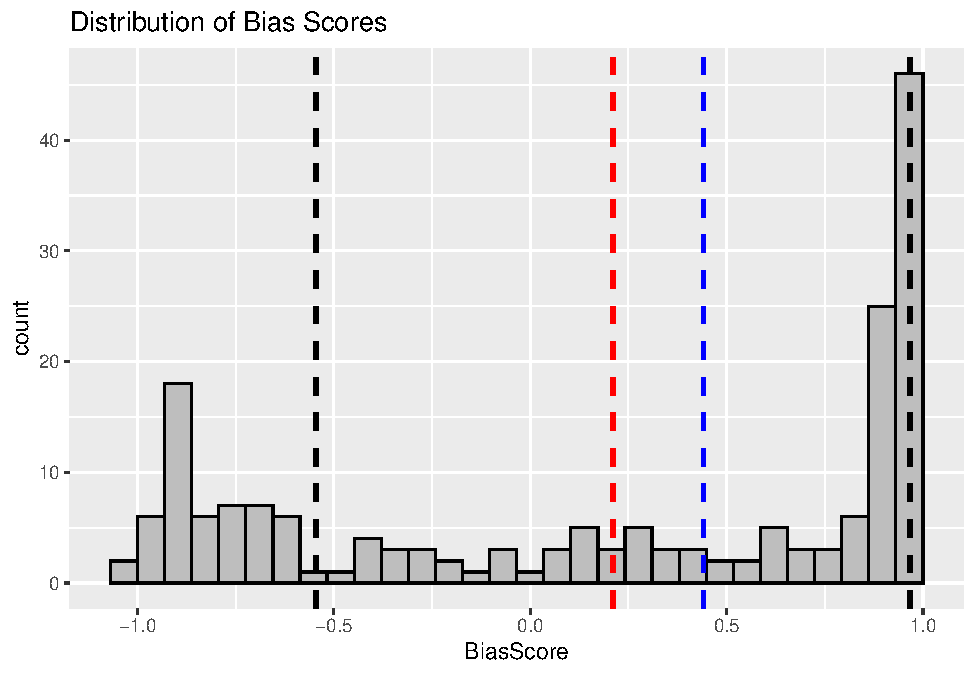
\includegraphics{MaiaAnalysis_2.15.24_files/figure-latex/bias_histo-1.pdf}

\begin{Shaded}
\begin{Highlighting}[]
\NormalTok{data }\SpecialCharTok{\%\textgreater{}\%}
  \FunctionTok{ggplot}\NormalTok{(}\FunctionTok{aes}\NormalTok{(}\AttributeTok{x=}\NormalTok{BiasScore)) }\SpecialCharTok{+}
  \FunctionTok{geom\_density}\NormalTok{(}\AttributeTok{fill =} \StringTok{"grey"}\NormalTok{, }\AttributeTok{color =} \StringTok{"black"}\NormalTok{) }\SpecialCharTok{+}
  \FunctionTok{ggtitle}\NormalTok{(}\StringTok{"Distribution of Bias Scores"}\NormalTok{)}
\end{Highlighting}
\end{Shaded}

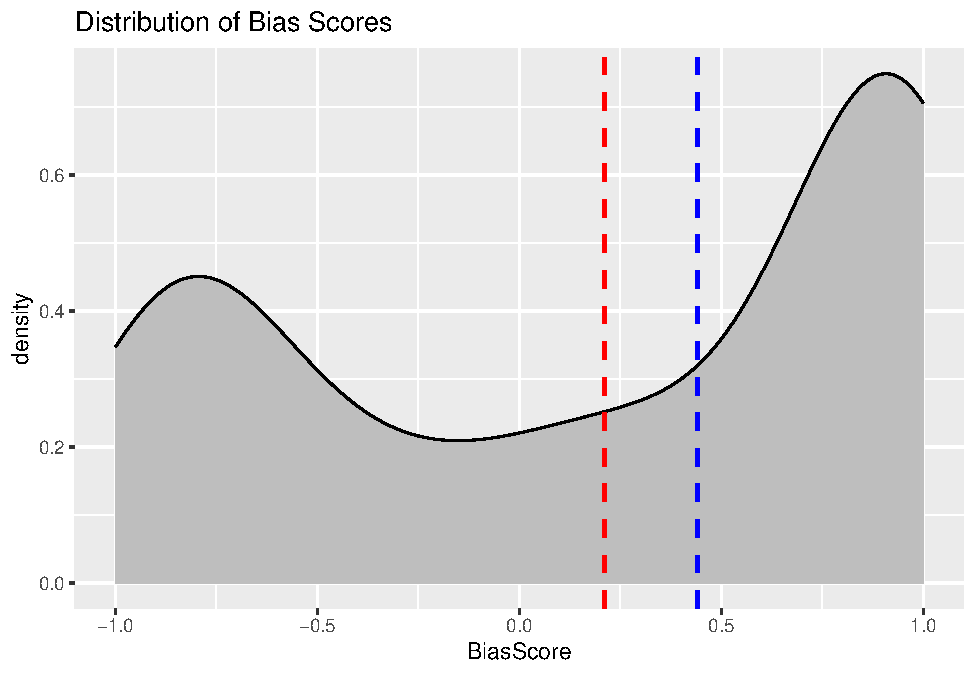
\includegraphics{MaiaAnalysis_2.15.24_files/figure-latex/bias_histo-2.pdf}

\begin{Shaded}
\begin{Highlighting}[]
\CommentTok{\# Split groups based on bias score}
\NormalTok{biased }\OtherTok{\textless{}{-}} \FunctionTok{subset}\NormalTok{(data, data}\SpecialCharTok{$}\NormalTok{BiasScore }\SpecialCharTok{\textgreater{}} \FloatTok{0.5} \SpecialCharTok{|}\NormalTok{ data}\SpecialCharTok{$}\NormalTok{BiasScore }\SpecialCharTok{\textless{}} \SpecialCharTok{{-}}\FloatTok{0.5}\NormalTok{)}
\NormalTok{neutral }\OtherTok{\textless{}{-}} \FunctionTok{subset}\NormalTok{(data, data}\SpecialCharTok{$}\NormalTok{BiasScore }\SpecialCharTok{\textless{}=} \FloatTok{0.5} \SpecialCharTok{\&}\NormalTok{ data}\SpecialCharTok{$}\NormalTok{BiasScore }\SpecialCharTok{\textgreater{}=} \SpecialCharTok{{-}}\FloatTok{0.5}\NormalTok{)}

\NormalTok{biased}\SpecialCharTok{$}\NormalTok{Group }\OtherTok{=} \StringTok{"biased"}
\NormalTok{neutral}\SpecialCharTok{$}\NormalTok{Group }\OtherTok{=} \StringTok{"neutral"}

\NormalTok{data\_grouped }\OtherTok{\textless{}{-}} \FunctionTok{rbind}\NormalTok{(biased, neutral)}

\NormalTok{data\_grouped }\SpecialCharTok{\%\textgreater{}\%}
  \FunctionTok{ggplot}\NormalTok{(}\FunctionTok{aes}\NormalTok{(}\AttributeTok{x =}\NormalTok{ BiasScore, }\AttributeTok{fill =}\NormalTok{ Group))}\SpecialCharTok{+}
  \FunctionTok{geom\_histogram}\NormalTok{()}
\end{Highlighting}
\end{Shaded}

\begin{verbatim}
## `stat_bin()` using `bins = 30`. Pick better value with `binwidth`.
\end{verbatim}

\includegraphics{MaiaAnalysis_2.15.24_files/figure-latex/bias_histo-3.pdf}

\begin{Shaded}
\begin{Highlighting}[]
\NormalTok{data\_grouped }\SpecialCharTok{\%\textgreater{}\%}
  \FunctionTok{ggplot}\NormalTok{(}\FunctionTok{aes}\NormalTok{(}\AttributeTok{x =}\NormalTok{ Incon.ConRT, }\AttributeTok{fill =}\NormalTok{ Group, }\AttributeTok{color =}\NormalTok{ Group))}\SpecialCharTok{+}
  \FunctionTok{geom\_histogram}\NormalTok{()}
\end{Highlighting}
\end{Shaded}

\begin{verbatim}
## `stat_bin()` using `bins = 30`. Pick better value with `binwidth`.
\end{verbatim}

\includegraphics{MaiaAnalysis_2.15.24_files/figure-latex/bias_histo-4.pdf}

\end{document}
